\documentclass[a4paper]{article}

\usepackage[english]{babel}
\usepackage[utf8]{inputenc}
\usepackage{fullpage}
\usepackage{amsmath}
\usepackage{graphicx}
\usepackage[colorinlistoftodos]{todonotes}
%\usepackage{hyperref}
\usepackage{amssymb}
\usepackage{subfigure}
\usepackage{url}
\usepackage[pagebackref=true,colorlinks,linkcolor=red,citecolor=green,breaklinks=true,bookmarks=false]{hyperref}
\usepackage{outline} 
\usepackage{pmgraph} \usepackage[normalem]{ulem}
\usepackage{graphicx} \usepackage{verbatim}
\usepackage{indentfirst}
\usepackage{listings}
\usepackage{xcolor}
\lstset{
	numbers=left, 
	numberstyle= \tiny, 
	keywordstyle= \color{ blue!70},
	commentstyle= \color{red!50!green!50!blue!50}, 
	frame=shadowbox, % 阴影效果
	rulesepcolor= \color{ red!20!green!20!blue!20} ,
	escapeinside=``, % 英文分号中可写入中文
	xleftmargin=2em,xrightmargin=2em, aboveskip=1em,
	framexleftmargin=2em
} 
\setlength{\parindent}{2em}
% \usepackage{minted} % need `-shell-escape' argument for local compile

\title{
	\vspace*{1in}
	
\includegraphics[width=2.75in]{figures/zhenglab-logo} \\
	\vspace*{1.2in}
	\textbf{\huge Weekly Work Report}
	\vspace{0.2in}
}

\author{Hongzhi Liu \\
	\vspace*{0.5in} \\
	\textbf{VISION@OUC} \\
	\vspace*{1in}
}

\date{\today}


\begin{document}
	\par
	\maketitle
	\setcounter{page}{0}
	\thispagestyle{empty}
	
	\newpage
	
	\section{Research problem}
	
	During this period of week, I spend time working about Faster R-CNN algorithm for off-line test and ROV equipment debugging in order to prepare URPC2018. Our team need to train 12 models that includes 11 kinds of image restoration and one image enhancement methods then output txt documents to evaluate algorithm performance with Yolo. Furthermore, I try to solve the error problems in running train code of flow-guided feature aggregation for video object detection.
	
	Because of difficulty in code modification, I have difficulty in adding codes to realize mirror reversal image as data sets in order to add training image. However, we realize that what should be tested are four-fifths picture of all data set in chronological order. Then, I spend much time modifying train.txt and test.txt. At last, I should try to test contest models with different threshold value to evaluate Faster RCNN algorithm. 
	
	\section{Research approach}
	
	In the process of research, I use the method of documentary analysis, comparative analysis and experimental research method. I read the thesis of Fast R-CNN \cite{Girshick2015Fast}, Faster R-CNN algorithm \cite{Ren2015Faster} and flow guided feature aggregation \cite{zhu17fgfa}. I try to unferstand core ideology in paper and learn about concept introduced by author.
	
	Besides, I learn grammatical application of python on the one hand, and on the other hand, I try to write code files to achieve the goal. By this method, I can have a better understanding of python.
	
	For deep learning, I watch the fifth course videos and write down the issues which I think are much important for further research. And then, I not only have learned the lessons of deep learning, but also put them into coding action. 
	
	
	\section{Research progress}
	
	During preparation for URPC2018, I collated several data sets to compare results of different methods for testing original graphs and evaluate how good the restoration algorithm are with mAP values. I continue to learn about Faster R-CNN algorithm \cite{Ren2015Faster} and relevant theory of flow guided feature aggregation \cite{zhu17fgfa}. Besides, I change the original image size to 256$\times$256 pixel and then resize to origin size. Then I use algorithm of python codes to complete the process of image mirror transformation. Furhtermore, Our team has carried out commissioning of ROV underwater equipment. And I will list details about weekly work in Tab.~\ref{t1} below.
	
	\begin{table}[hb]
		\centering
		\caption{Weekly work progress.}
		\begin{tabular}{c|p{10cm}}
			\hline 
			& Finish collatting several data sets to train contest model.\\
			
			& Finish comparing results of different methods. \\
			
			URPC2018 & Finish training a lot of model evaluation data with different threshold.\\
			
			& Finish comparing mAP value of different methods and judge which are better.\\
			
			& Finish debugging ROV equipment.\\
			\hline
			Deep Learning& Finish learning Sequence Models which is the fifth course of deep learning.\\
			\hline
		\end{tabular}
		\label{t1}
	\end{table} 
	
	\section{Progress in this week}
	
	During preparation for URPC2018, I have collated several data sets to train contest model. Then I use algorithm to complete the process of image mirror transformation. Besides, I test origin image models and obtain mAP value with different thresholds. Furthermore, our team carry out commissioning of ROV underwater equipment.  
	\begin{description}
		\item[Step 1] Finish collatting several data sets to train contest model.
		\item[Step 2] Finish training a lot of model evaluation data with different threshold.
		\item[Step 3] Finish comparing mAP value of different methods and judge which are better.
		\item[Step 4] Finish debugging ROV equipment.\label{t2}
	\end{description}
	
	\subsection{Training Data Sets}
	
	In this week, I have collated several data sets to train contest model and compare results of different methods for testing original graphs, which can better evalute performance of Faster RCNN algorithm. According to the teacher's request, I should train origin images and their mirror convert pictures first as seen in Fig.~\ref{p1}. The two pictures are symmetrical in the axis of the mirror. This can be regarded as an effective way of image enhancement. Besides, I change the original image size to 256$\times$256 pixel and then resize to origin size following recommendation of the teacher as seen in Fig.~\ref{p2}.
	\begin{figure}
		\begin{center}
			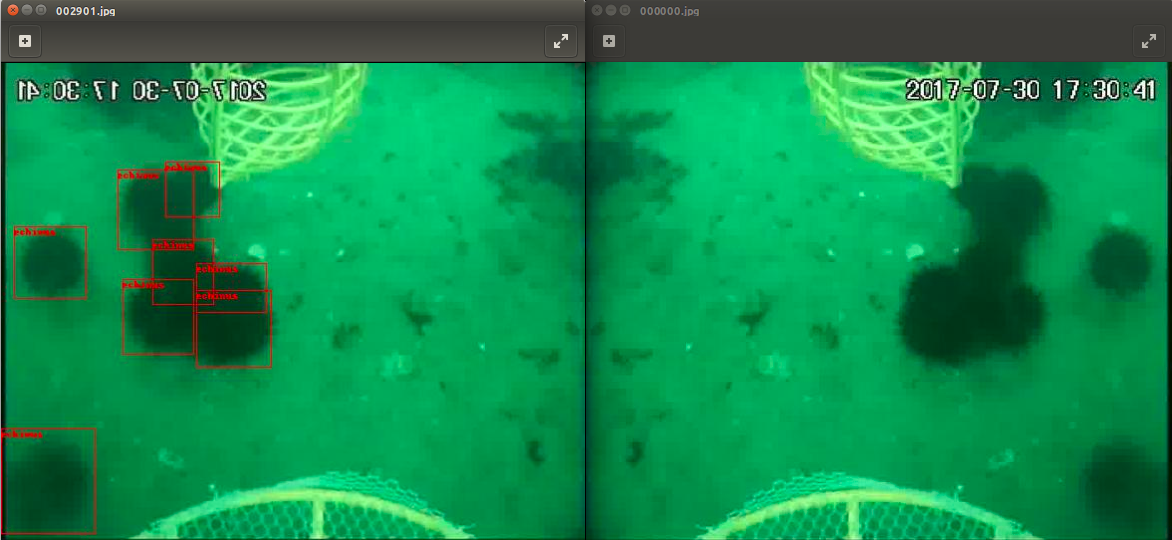
\includegraphics[scale=0.35]{figures/1.png} 
		\end{center}
		\caption{Data sets of picture mirror overturn method.}
		\label{p1}
	\end{figure}
	
	\begin{figure}
		\begin{center}
			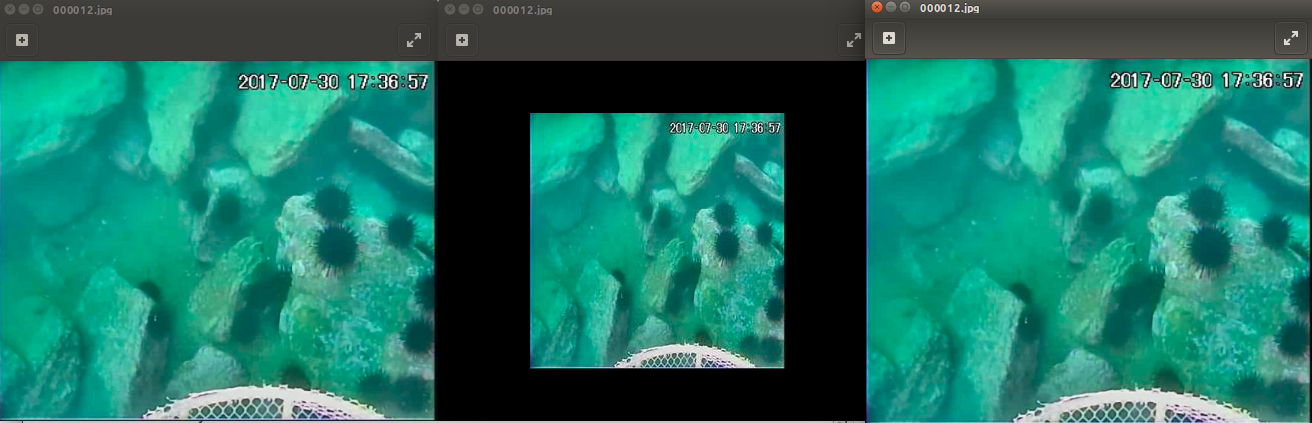
\includegraphics[scale=0.35]{figures/2.png} 
		\end{center}
		\caption{Data sets of resizing origin images.}
		\label{p2}
	\end{figure}
	
	Coordinate position of bounding box after mirror transformation can be obtained by Eq.~\ref{q1} if knowing the width and height of every picture in data sets. Then I use Algorithm~\ref{g1} to complete the process of image mirror transformation. Besides, I realize that this conversion, in turn, would require changes to all xml files for training models, so I use Algorithm~\ref{g2} to modified coordinates of bounding boxes such as xmin and ymin.
	\begin{equation}
	\begin{cases}
	xmin = width-xmax\\
	ymin =ymin\\
	xmmax = width-xmin\\
	ymax = ymax\\
	\end{cases} \label{q1}
	\end{equation}
	
\lstset{language=python}
\begin{lstlisting}
set -e  # or use "set -o errexit" to quit on error.
set -x  # or use "set -o xtrace" to print the statement 
before you execute it.	
FILES=*.jpg
for f in $FILES
do
echo "$f"
convert $f -flop $f
done
\end{lstlisting}\label{g1}
	
\lstset{language=python}
\begin{lstlisting}
# coding:utf-8
import math
import numpy as np
import xml.etree.ElementTree as ET
import os
	
xmlpath = './5801xml/'         
rotated_xmlpath = 'rotatedxml'
for i in os.listdir(xmlpath):
print(i)
a, b = os.path.splitext(i)  
print(a,b)                          
tree = ET.parse(xmlpath + a + '.xml')
root = tree.getroot()
for ch in root.iter('size'):
width = float(ch.find(width).text)
for box in root.iter('bndbox'):
xmin = float(box.find('xmin').text)
ymin = float(box.find('ymin').text)
xmax = float(box.find('xmax').text)
ymax = float(box.find('ymax').text)
box.find('xmin').text = str(width-xmax)
box.find('ymin').text = str(ymin)
box.find('xmax').text = str(width+xmin)
box.find('ymax').text = str(ymax)
tree.write(rotated_xmlpath + a + '_' +'d.xml')
print(str(a) + '.xml has been rotated for  '+'°')
\end{lstlisting}\label{g2}
	
	\subsection{Test Contest Models}
	
	After a period of training and testing several models, I get a lot of model evaluation data with 0.8 threshold, but are far from enough. So I test origin image models and obtain mAP value with different thresholds which can be seen in Fig.~\ref{p3}. We can see from the picture that mAP value increases with decreasing threshold. 
	
	\begin{figure}
		\begin{center}
			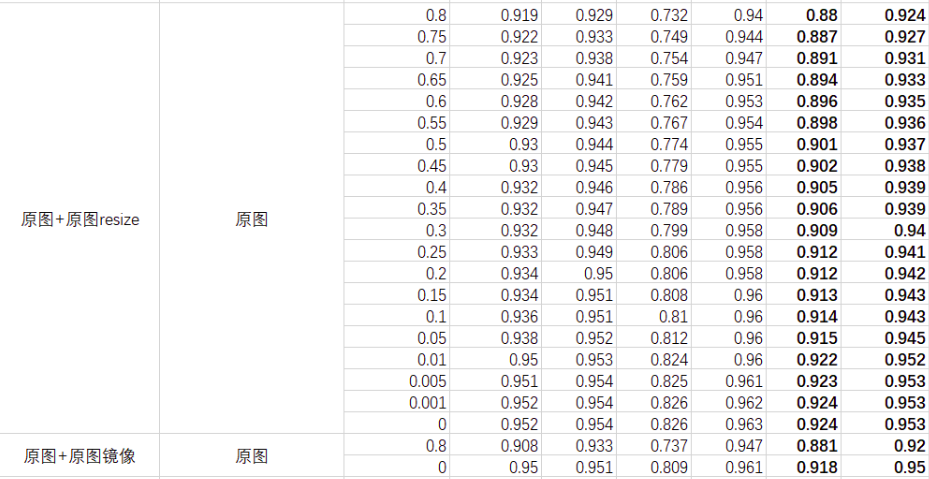
\includegraphics[scale=0.5]{figures/3.png}
		\end{center}
		\caption{Output results of two model. The first column is threshold. Then the four columns representative holothurian, echinus, scallop and starfish. The sixth column is mAP value.}
		\label{p3}
	\end{figure}
	
	After I train a contest model with on-line data sets, I find the output result is not very good as shown in Fig.~\ref{p5}. So we check xml files and label numbers to train again.
	\begin{figure}
		\begin{center}
			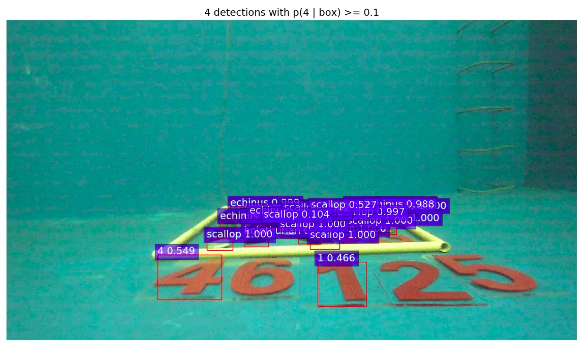
\includegraphics[scale=0.5]{figures/10.png}
		\end{center}
		\caption{Output result picture of contest model with on-line data sets.}
		\label{p5}
	\end{figure}
	
	\begin{figure}
		\centering 
		\subfigure[]{ 
			\label{p4a} %% label for first subfigure 
			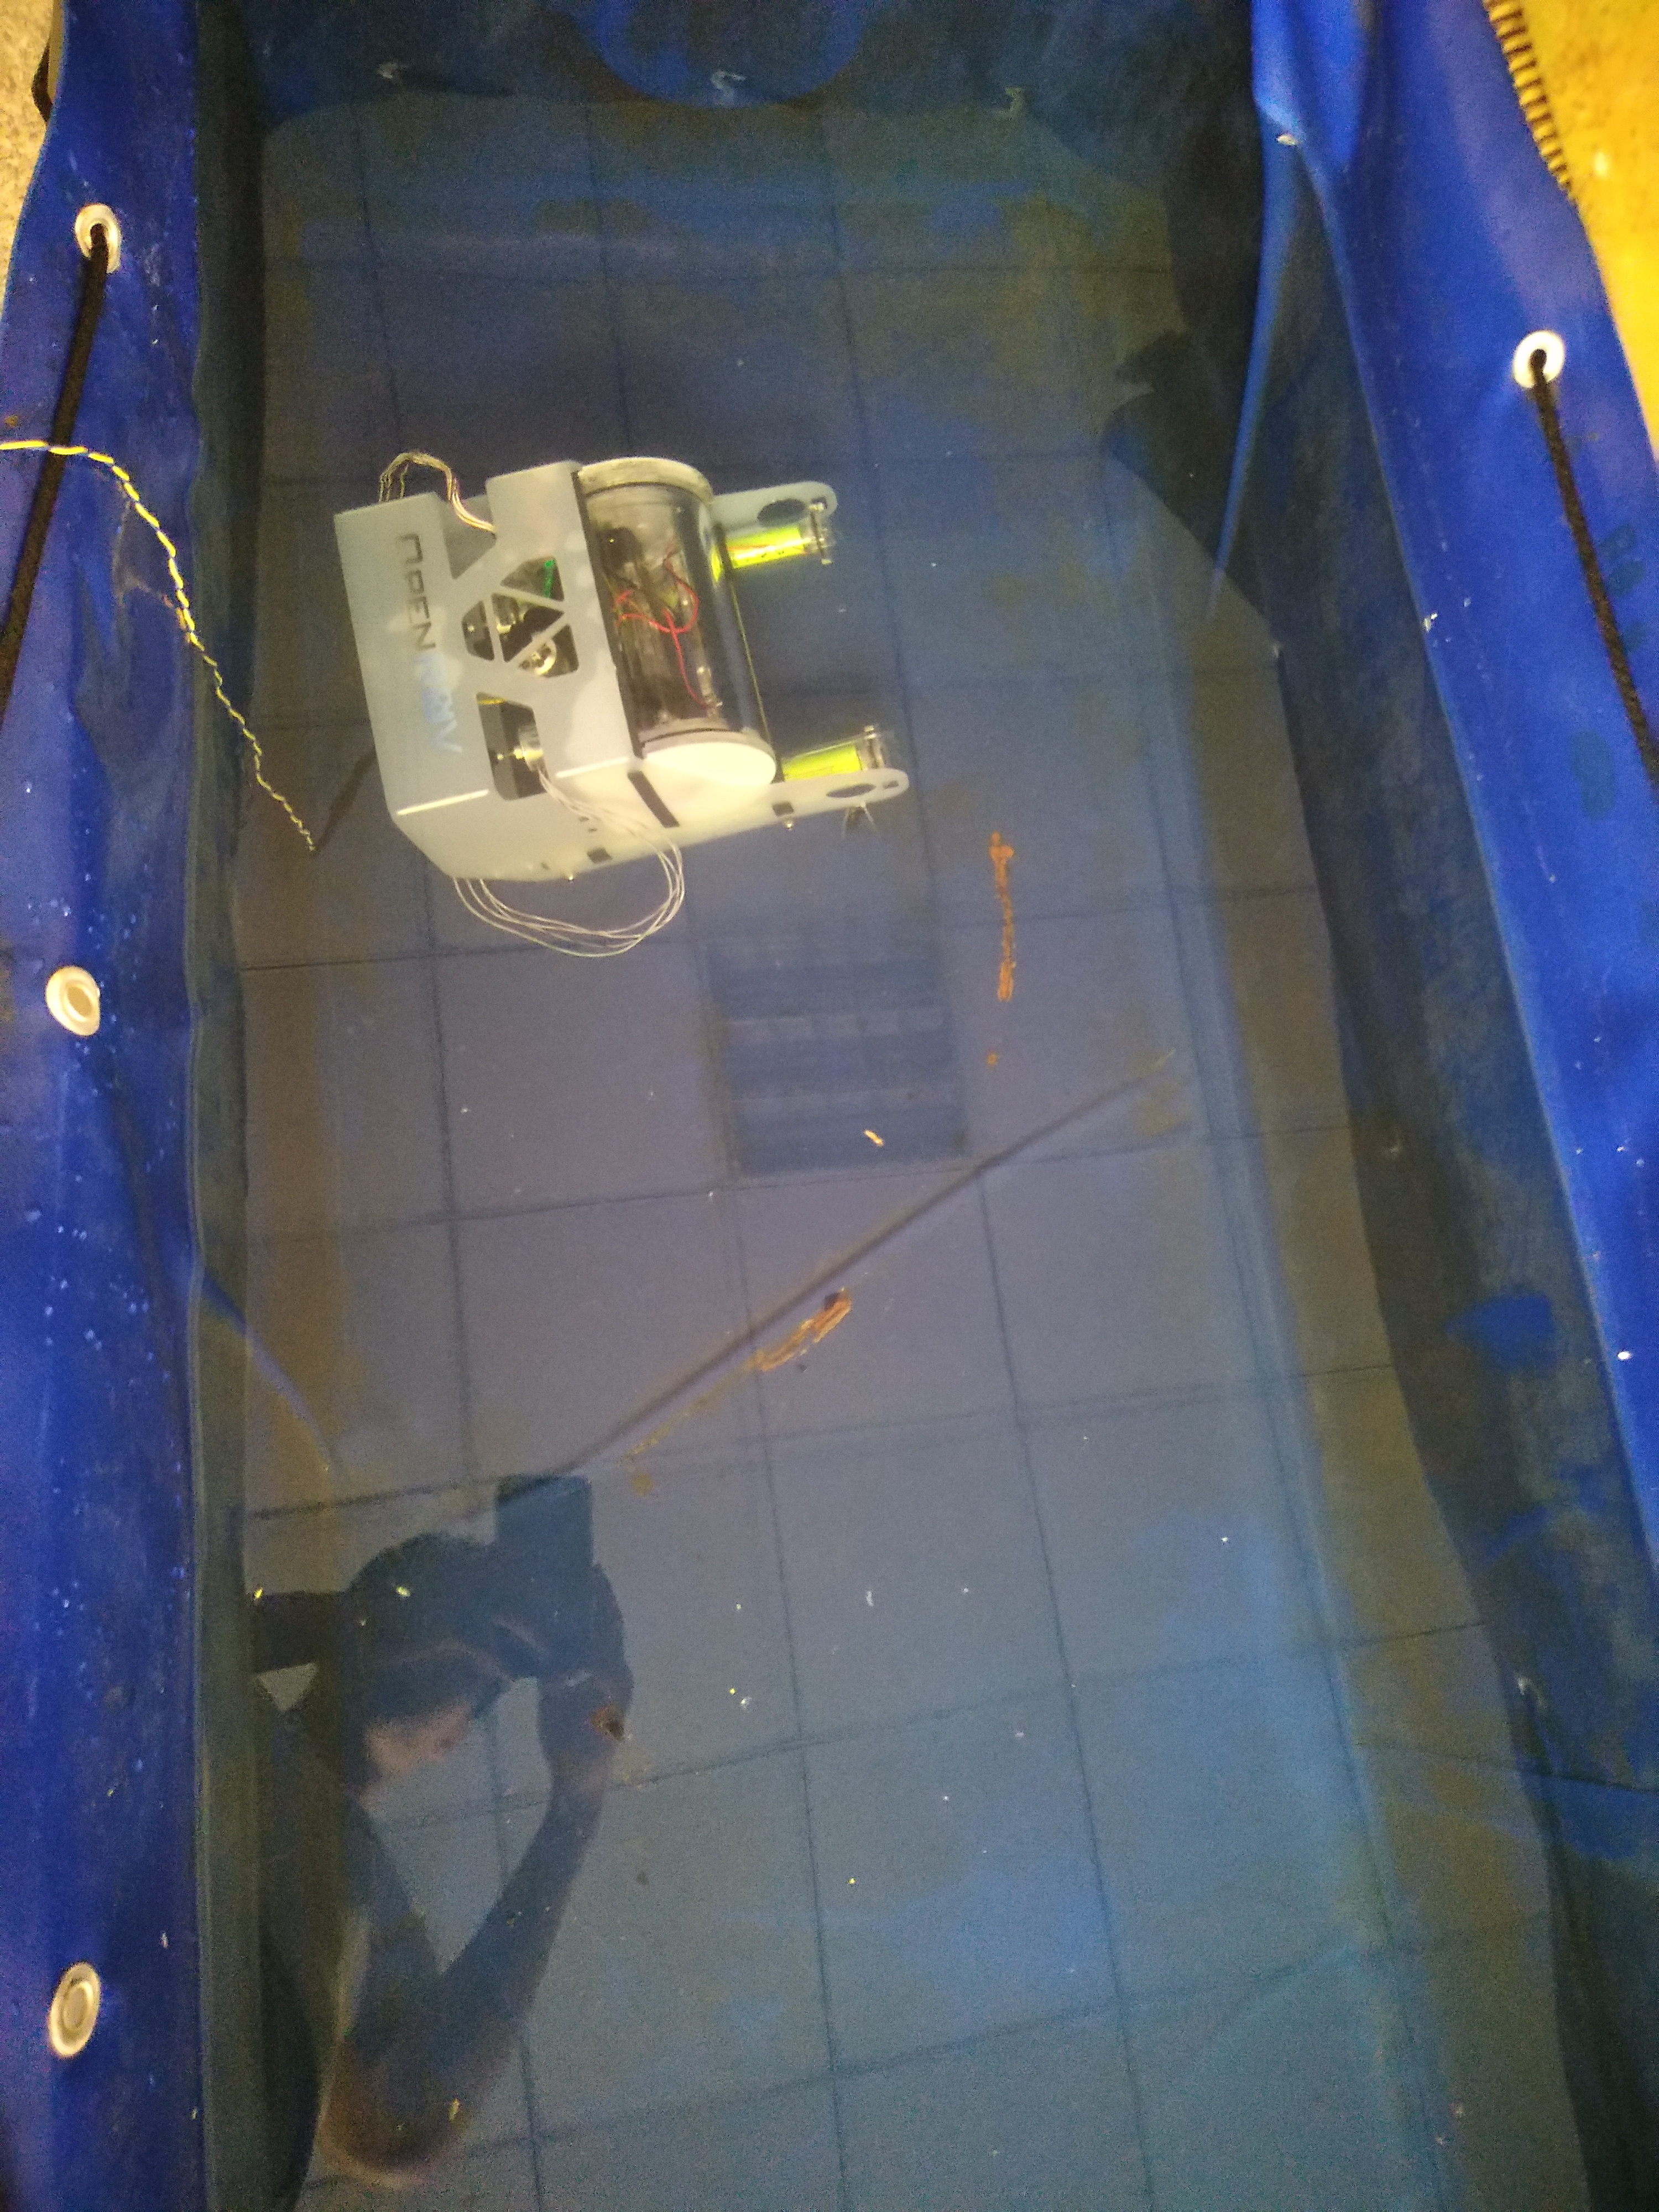
\includegraphics[width=7cm]{figures/8.jpg} 
		} 
		\subfigure[]{ 
			\label{p4b} %% label for second subfigure 
			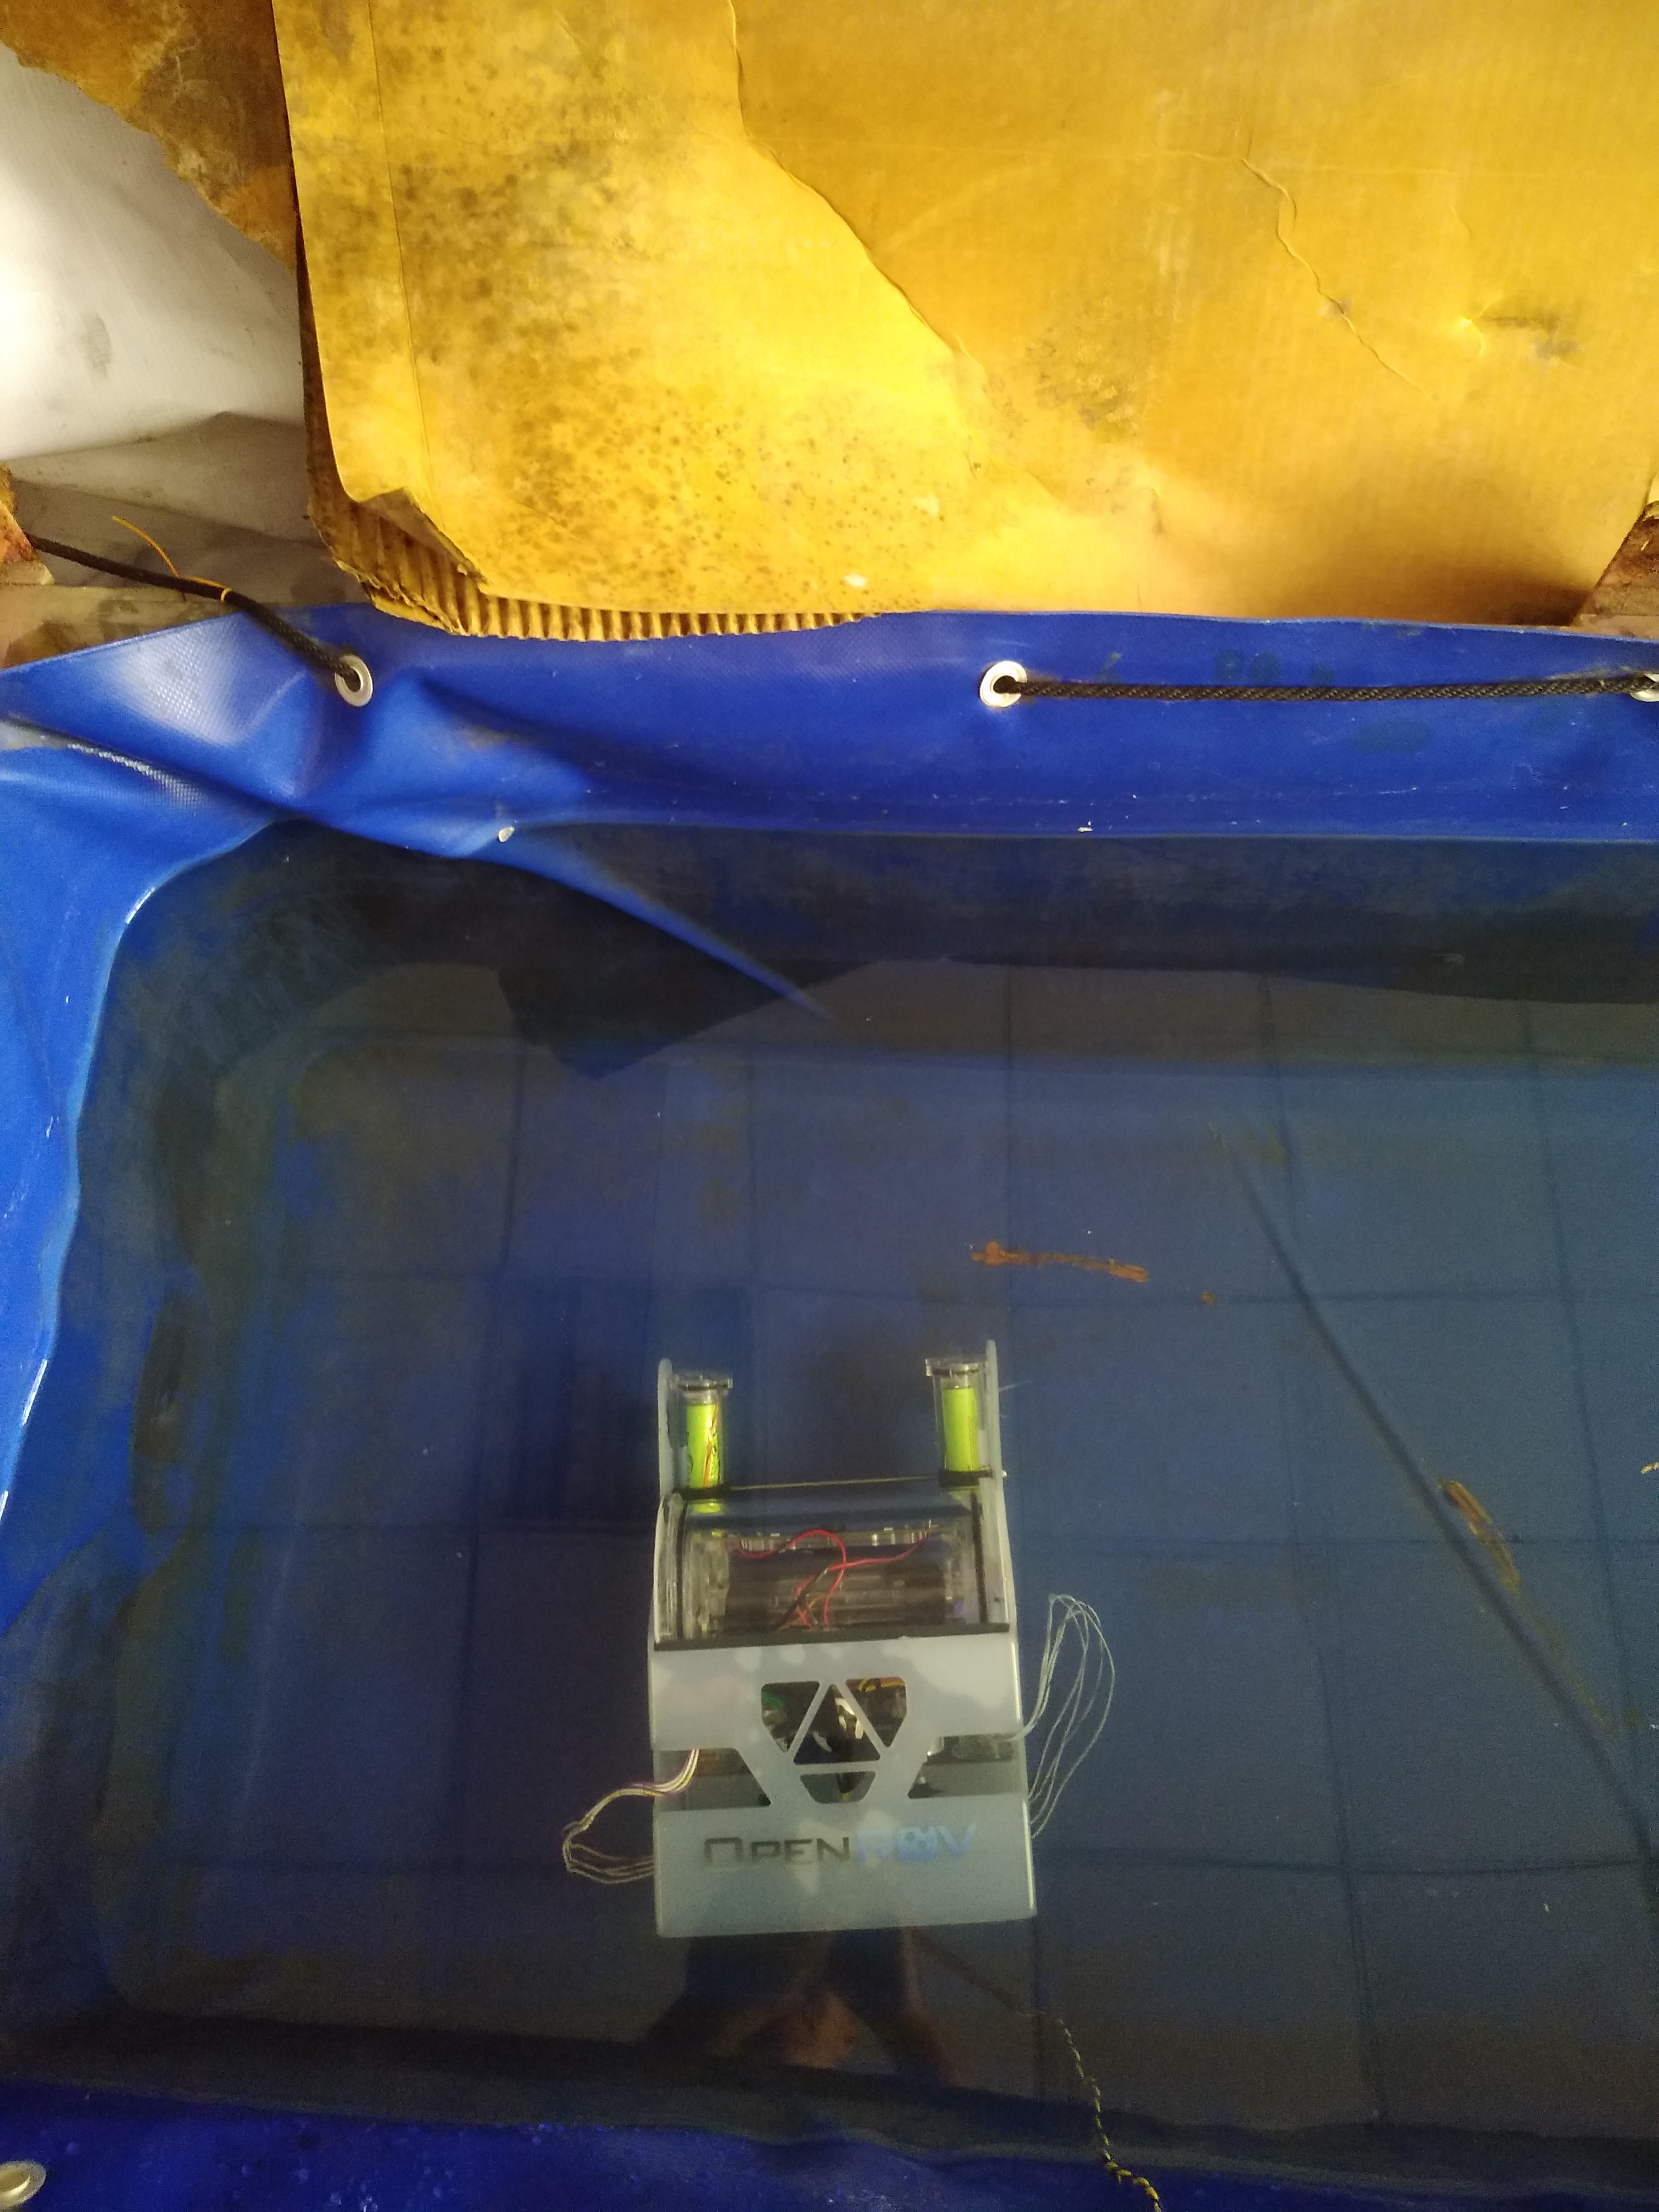
\includegraphics[width=7cm]{figures/9.jpg} 
		} 
		\caption{ROV equipment on-site commissioning process.} 
		\label{p4} %% label for entire figure 
	\end{figure}
	
	\lstset{language=python}
	\begin{lstlisting}
	def demo(sess, net, image_name):
	# Load the demo image
	print('demoDemo for data/demo/{}{}'.format(im_name[0], '.jpg'))
	print('demoDemo for data/demo/{}{}'.format(im_name[1], '.jpg'))
	print('\n')
	
	all_name = image_name+'.jpg'
	im_file = os.path.join(cfg.DATA_DIR, 'demo', all_name)
	im = cv2.imread(im_file)
	
	fr = open('/home/henry/Files/tf-faster-rcnn-contest/data/
	VOCdevkit2007/test_list.txt', 'r')
	for im_name in fr:
	im_name = im_name.strip()
	im_name = im_name.split(' ')
	print('~~~~~~~~~~~~~~~~~~~~~~~~~~~~~~~~~~~')
	print('mainDemo for data/demo/{}{}'.format(im_name[0],'.jpg'))
	print('mainDemo for data/demo/{}{}'.format(im_name[1],'.jpg'))
	print('\n')
	demo(sess, net, im_name[0])
	\end{lstlisting}\label{g8}
	
	\subsection{ROV Equipment Debugging}
	
	Our team has carried out commissioning of ROV underwater equipment this week as Fig.~\ref{p4}. We encountered many problems when we debugged the device. 	First of all, steering gear turns opposite and we change the battery and work well. Then we adjust the direction of the camera and can get image from camera. Furthermore, what we need to do next step is equipment and program docking, which decides whether to win or lose the contest.
	
	
	
	\section{Plan}
	
	\begin{tabular}{rl}
		\textbf{Objective:} & Finish off-line and on-line test for 2018URPC. \\
		\textbf{Deadline:} & 2018.08.31
	\end{tabular}
	
	\begin{description}
		\item[\normalfont 2018.08.27---2018.09.02] Finish preparation for 2018URPC.
		\item[\normalfont 2018.09.03---2018.09.09] Finish literature review about image synthesis.
		\item[\normalfont 2018.09.10---2018.09.16] Finish reading reference documentation.
	\end{description}
	
	
	
	% If you don't cite any references, please comment the following two lines
	\bibliographystyle{ieee}
	\bibliography{ref.bib}
	
\end{document}